\documentclass[a4paper,10pt]{article}

\usepackage[brazilian]{babel}
\usepackage[utf8]{inputenc}
\usepackage[T1]{fontenc}
\usepackage{titlesec}
\usepackage{graphicx}
\usepackage{mathtools}
\usepackage{amsthm}
\usepackage[top=1.0in,bottom=1.0in]{geometry}

\titleformat{\section}
  {\normalfont\scshape\bfseries}{\thesection}{1em}{}
\titleformat{\subsection}
  {\normalfont\scshape\bfseries}{\thesubsection}{1em}{}
\titleformat{\paragraph}
  {\normalfont}{\theparagraph}{1em}{}

\theoremstyle{plain}

\newtheorem*{spn-def}{Definição}

\title{\textbf{Aprendizado Automático de Sum-Product Networks (SPN)}}

\begin{document}
\date{}
\author{}
\vspace*{-40pt}
{\let\newpage\relax\maketitle}

Projeto de MAC0215 (Atividade Curricular em Pesquisa)

Aluno: Renato Lui Geh (Bacharelado em Ciência da Computação)

Orientador: Denis Deratani Mauá

\section{Proposta}

\paragraph{
  O objetivo deste projeto é realizar uma comparação das principais técnicas de aprendizado 
automático de Sum-Product Networks a partir de um conjunto de dados, avaliando o desempenho 
e os resultados das técnicas utilizadas.
}

\section{Projeto}
\subsection{Definição}

\paragraph{
  Sum-Product Networks são uma nova classe de modelos probabilísticos cuja inferência é sempre
tratável.
}

\begin{spn-def} Uma SPN é:

\begin{enumerate} \itemsep0pt
  \item Uma distribuição univariante tratável.
  \item Um produto de SPNs cujos escopos são disjuntos.
  \item Uma soma de SPNs com peso não negativo cujos elementos tem mesmo escopo.
  \item Nada mais é uma SPN.
\end{enumerate}
\end{spn-def}

\paragraph{
  Podemos definir graficamente uma SPN como um grafo enraizado, direcionado e acíclico onde as 
folhas são sempre variáveis (ou distribuições univariantes), seus nós internos são somas ou 
produtos e para todo vértice conectando um nó soma com um nó filho há um peso não negativo. 
Também assume-se que toda soma e produto estão em alturas alternantes, ou seja, todo nó pai 
de um nó interno que é soma é um produto e vice-versa.
}

\begin{figure}[h]
\centering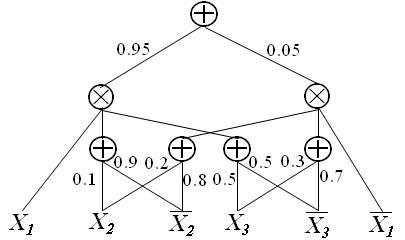
\includegraphics[scale=0.7]{imgs/domingos_poon.jpg}
\caption{Um exemplo de uma SPN com variáveis Booleanas, onde $x_1,...,x_d$ e 
  $\overline{x_1},...,\overline{x_d}$ são folhas e o resto dos nós são somas ou produtos.
    [Domingos Poon]}
\end{figure}

\subsection{Características}

\paragraph{
  Há várias vantagens de SPNs sobre outras redes de aprendizado:
}

\begin{enumerate} \itemsep0pt
  \item Estudos mostram que SPNs tem estrutura parecida a Modelos Gráficos Probabilisticos (PGM), 
    mas inferência é mais rápida e precisa em dependências com grande largura. [Gens Domingos]
  \item SPNs apresentam inferência mais rápida comparado a Redes Bayesianas, cuja inferência é
    NP-difícil.
  \item Experimentos mostram que aprendizado de arquiteturas SPN tiveram melhores resultados quando
    comparadas a outras arquiteturas estáticas. [Clustering Dennis Ventura]
\end{enumerate}

\subsection{Aplicações}

SPNs obtiveram resultados impressionantes em muitos conjuntos de dados, tais como:

\begin{itemize} \itemsep0pt
  \item Reconstrução de imagens.
  \item Classificação.
  \item Reconhecimento de atividade.
  \item Logs click-through.
  \item Sequências de ácido nucleico.
  \item Filtragem colaborativa.
\end{itemize}

\end{document}
